
%% bare_jrnl.tex
%% V1.3
%% 2007/01/11
%% by Michael Shell
%% see http://www.michaelshell.org/
%% for current contact information.
%%
%% This is a skeleton file demonstrating the use of IEEEtran.cls
%% (requires IEEEtran.cls version 1.7 or later) with an IEEE journal paper.
%%


\documentclass[journal]{IEEEtran}
%
% If IEEEtran.cls has not been installed into the LaTeX system files,
% manually specify the path to it like:
% \documentclass[journal]{../sty/IEEEtran}


%%%%%%%%%%%%%%%%%%%%%%%
\usepackage[]{graphicx}

%%%%%%%%%%%%%%%%%%%%%%%%%%%%%%%%%%%%%%%%%%%%%%%%%%%%%%%%%%%%%%%%%%%%%%%%%%%%%%%%%%

\usepackage[svgnames]{xcolor} % Enabling colors by their 'svgnames'

\usepackage{amsmath}
\usepackage{amsfonts}
\usepackage{amssymb}

% correct bad hyphenation here
\hyphenation{op-tical net-works semi-conduc-tor}

\newtheorem{mydef}{Definition}
\newtheorem{corollary}{Corollary}[theorem]

\begin{document}
%
% paper title
% can use linebreaks \\ within to get better formatting as desired
\title{ Error Reduction in the Tuning of Six Hole's Ocarina }
%
%

\author{Fernando Pujaico Rivera% <-this % stops a space
%\thanks{Los amigos que me regalaron la arcilla}% <-this % stops a space
%\thanks{Los amigos que me orientaron en la construccion.}% <-this % stops a space
%\thanks{Las personas que dedicaron tiempo al planteo de reglas fisicas para la ocarina}
}



% The paper headers
\markboth{Journal of \LaTeX\ Class Files,~Vol.~1, No.~1, Junio~2010}%
{Shell \MakeLowercase{\textit{et al.}}: Bare Demo of IEEEtran.cls for Journals}
% The only time the second header will appear is for the odd numbered pages
% after the title page when using the twoside option.
% 
% *** Note that you probably will NOT want to include the author's ***
% *** name in the headers of peer review papers.                   ***
% You can use \ifCLASSOPTIONpeerreview for conditional compilation here if
% you desire.



% make the title area
\maketitle


\begin{abstract}
In this work is proposed a method of frequency tuning with minimum error in the six hole's ocarinas,
It will be based in a minimization rule proposed in this work.
The error in all notes was obtained and it is compared with the error produced 
in a process tuning case.
\end{abstract}
% IEEEtran.cls defaults to using nonbold math in the Abstract.
% This preserves the distinction between vectors and scalars. However,
% if the journal you are submitting to favors bold math in the abstract,
% then you can use LaTeX's standard command \boldmath at the very start
% of the abstract to achieve this. Many IEEE journals frown on math
% in the abstract anyway.

% Note that keywords are not normally used for peerreview papers.
\begin{IEEEkeywords}
ocarina, tuning.
\end{IEEEkeywords}






% For peer review papers, you can put extra information on the cover
% page as needed:
% \ifCLASSOPTIONpeerreview
% \begin{center} \bfseries EDICS Category: 3-BBND \end{center}
% \fi
%
% For peerreview papers, this IEEEtran command inserts a page break and
% creates the second title. It will be ignored for other modes.
\IEEEpeerreviewmaketitle



\section{Introduction}

\IEEEPARstart{E}{l}  estilo de dedillado de la ocarina tipo pendiente fue desarrollado en 1960
por John Taylor \cite{JohnTaylorRef} ; el y Barry Jennings \cite{BarryJenningsRef} impulsaron 
y difundieron este estilo.


\section{Math and music}
In this paper It is used a tuning method with 12 tone equal temperament; thus, the frequency interval
between any pair of adjacent notes has the same ratio $\rho = {\sqrt[12]{2}}$.
The Table \ref{tab:notes} shows as the musical notes from $C$ until $\bar{D}$
are  distributed, where $f_0$ represent the frequency of $C$ note and the next notes
follow the progression ${\rho}^i f_{0}$ with $i$ representing the separation degree with $C$. 

\begin{table}[h]
\center
{\renewcommand{\arraystretch}{1.5}
\begin{tabular}{c|c|c|c|c|c|c|c}
\hline
$C$ & $C\#$ & $D$ & $D\#$ & $E$ & $F$ & $F\#$ & $G$ \\ \hline
$f_{0}$ & ${\rho}^1 f_{0}$ & ${\rho}^2 f_{0}$ & ${\rho}^3 f_{0}$ & ${\rho}^4 f_{0}$ & ${\rho}^5 f_{0}$ & ${\rho}^6 f_{0}$ & ${\rho}^7 f_{0}$  \\
\hline \hline 
$G\#$ & $A$ & $A\#$ & $B$ & $\bar{C}$ & $\bar{C}\#$ & $\bar{D}$  & ~\\ \hline
${\rho}^8 f_{0}$ & ${\rho}^9 f_{0}$ & ${\rho}^{10} f_{0}$ & ${\rho}^{11} f_{0}$ & ${\rho}^{12} f_{0}$ & ${\rho}^{13} f_{0}$ & ${\rho}^{14} f_{0}$ & ~\\ 
\hline
\end{tabular}
}
\caption{Musical notes}
\label{tab:notes}
\end{table}

\begin{mydef}
Known the frequency relation between the notes, will be defined the variable $\hat{z}_i=\left( {\rho}^{i} f_0 \right)^{2} $,
so that the  column vector $\mathbf{\hat{z}}$ is represented as in the Eq. \ref{eq:vecz}.
\begin{equation} \label{eq:vecz}
\mathbf{\hat{z}}
= \left( \hat{z}_1, \hat{z}_2, \hat{z}_3, \hdots, \hat{z}_{14}\right)^{T}
\end{equation}
 
\end{mydef}

\subsection{The maximum accepted tuning error}
To obtain the percent value of the maximum accepted tuning error ($\delta_{max}$),
It is necessary to use the fact that between any two consecutive notes with frequencies
$f_a$ and $\rho f_a$, exist a proportion of $\rho=1.059463$, this mean
that the next consecutive note is ever a $+5.9463\%$ that the last note. So that,
the maximum accepted tuning error in a note, 
to avoid a recognition mistake, it is equal to $\delta_{max} = \pm 2.9731\% \equiv (\rho-1)/2$.



\section{Fingering chart in  6 hole's ocarina}
The Fig. \ref{fig:ocarinaview} represents the hole distribution in the ocarina
used in this work; where $S_0$ represent the sound hole (voicing)
and the holes $S_1$, $S_2$, $S_3$, ... and $S_6$ represent the tune holes.
\begin{figure}[ht!]
\centering
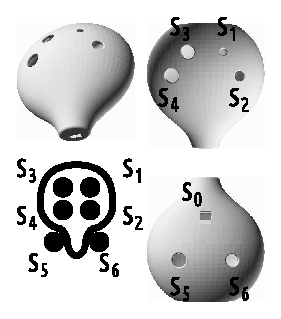
\includegraphics[width=0.50\columnwidth]{ocarina-view.eps}
\caption{View of 6 hole ocarina. }
\label{fig:ocarinaview}
\end{figure}
The fingering chart used in this ocarina model is based in the 
fingering style proposed by John Taylor \cite{JohnTaylorRef}. In the
Table \ref{table:chart} we can see the fingering chart that indicates the configuration of open or close holes
to produce the tones from $C$ until $\bar{D}$, where a value $S_i=1$ represents an
open hole and the value $S_i=0$ a closed hole.
\begin{table}[h]
\center
\begin{tabular}{l|c|c|c|c|c|c}
Note & $S_1$ & $S_2$ & $S_3$ & $S_4$ & $S_5$ & $S_6$ \\ \hline
\hline 
$C$  & 0 & 0 & 0 & 0 & 0 & 0 \\
$C\#$& 0 & 0 & 0 & 0 & 0 & 1 \\
$D$  & 1 & 0 & 0 & 0 & 0 & 0 \\
$D\#$& 1 & 0 & 0 & 0 & 0 & 1 \\
$E$  & 0 & 1 & 0 & 0 & 0 & 0 \\
$F$  & 1 & 1 & 0 & 0 & 0 & 0 \\
$F\#$& 0 & 0 & 1 & 0 & 0 & 0 \\
$G$  & 1 & 0 & 1 & 0 & 0 & 0 \\
$G\#$& 0 & 1 & 1 & 0 & 0 & 0 \\
$A$  & 1 & 1 & 1 & 0 & 0 & 0 \\
$A\#$& 1 & 0 & 1 & 1 & 0 & 0 \\
$B$  & 0 & 1 & 1 & 1 & 0 & 0 \\
$\bar{C}$& 1 & 1 & 1 & 1 & 0 & 0 \\
$\bar{C}\#$& 0 & 1 & 1 & 1 & 1 & 0 \\
$\bar{D}$& 1 & 1 & 1 & 1 & 1 & 0 \\ 
\hline 
\end{tabular}
\caption{Fingering chart}
\label{table:chart}
\end{table}

\section{Resonance frequency in ocarinas}
Subsection text here.

\begin{equation} \label{EcA}
 f = \frac{c}{2 \pi} \sqrt{\frac{\frac{A_{0}S_{0}}{l_{0}}+\frac{A_{1}S_{1}}{l_{1}}+\frac{A_{2}S_{2}}{l_{2}}+ . . .}{V} }   
\end{equation}


\subsection{Reordering the resonance equation}
\begin{equation} \label{EcC}
 h_{i} =  \left( \frac{c^2}{4 {\pi}^2 V}\right) \left( \frac{A_{i}}{l_{i}}    \right)
\end{equation}

\begin{equation} \label{EcD}
 f^{2} = \sum_{i}{S_i h_i}
\end{equation}

\begin{corollary}

\begin{equation} 
 f_0^{2} = h_0
\end{equation}
 
\end{corollary}



\subsection{Planteamiento del problema}



\begin{equation}
\mathbf{z}
=  
\begin{bmatrix}
1 \\ 
1 \\ 
1 \\ 
1 \\ 
1 \\ 
1 \\ 
1 \\
1 \\ 
1 \\ 
1 \\ 
1 \\ 
1 \\ 
1 \\ 
1
\end{bmatrix}
h_{0} + 
\begin{bmatrix}
0 & 0 & 0 & 0 & 0 & 1 \\
1 & 0 & 0 & 0 & 0 & 0 \\
1 & 0 & 0 & 0 & 0 & 1 \\
0 & 1 & 0 & 0 & 0 & 0 \\ 
1 & 1 & 0 & 0 & 0 & 0 \\ 
0 & 0 & 1 & 0 & 0 & 0 \\
1 & 0 & 1 & 0 & 0 & 0 \\ 
0 & 1 & 1 & 0 & 0 & 0 \\ 
1 & 1 & 1 & 0 & 0 & 0 \\ 
1 & 0 & 1 & 1 & 0 & 0 \\ 
0 & 1 & 1 & 1 & 0 & 0 \\ 
1 & 1 & 1 & 1 & 0 & 0 \\
0 & 1 & 1 & 1 & 1 & 0 \\
1 & 1 & 1 & 1 & 1 & 0 
\end{bmatrix} 
\begin{bmatrix}
h_{1} \\
h_{2} \\
h_{3} \\
h_{4} \\
h_{5} \\
h_{6}
\end{bmatrix} 
\end{equation}


\begin{equation}
\mathbf{z}(h) =  \mathbf{L}h_0 +  \mathbf{A} \mathbf{h}
\end{equation}


\section{minimizacion de errores}

\begin{equation}
e^2= || \mathbf{\hat{z}} - \mathbf{z}(\mathbf{h}) ||^2
\end{equation}

\begin{equation}
\mathbf{h}^{*}=
 \left(\mathbf{A}^T\mathbf{A}\right)^{-1}\mathbf{A}^T
 \left(\mathbf{P}-\mathbf{L}\right)
h_0
\end{equation}

\begin{equation}
\mathbf{z}^{*}=
\left(\mathbf{L}
+\mathbf{A}\left(\mathbf{A}^T\mathbf{A}\right)^{-1}\mathbf{A}^T
 \left(\mathbf{P}-\mathbf{L}\right) \right)
f_0^2
\end{equation}

\subsection{cuadro comparativo}
Subsubsection text here.





\section{Resultados}

En la Tabla \ref{table:res}

\begin{table}[h]
\center
\begin{tabular}{c|c|c|c}
Note & temperada (hz)& optima (hz) & Error \% of $|\delta_{max}| $ \\ \hline
\hline 
$C$  & 1.0000$f_0$ & 1.0000$f_0$ & 0.00000\%$/\delta_{max}$ \\
$D$  & 1.1225$f_0$ & 1.1330$f_0$ & 0.93497\%$/\delta_{max}$ \\
$E$  & 1.2599$f_0$ & 1.2454$f_0$ & 1.15501\%$/\delta_{max}$ \\
$F$  & 1.3348$f_0$ & 1.3544$f_0$ & 1.46910\%$/\delta_{max}$ \\
$G$  & 1.4983$f_0$ & 1.5037$f_0$ & 0.36193\%$/\delta_{max}$ \\
$A_2$& 1.6818$f_0$ & 1.6769$f_0$ & 0.28820\%$/\delta_{max}$ \\
$B_2$& 1.8877$f_0$ & 1.9079$f_0$ & 1.06636\%$/\delta_{max}$ \\
$C_2$& 2.0000$f_0$ & 1.9808$f_0$ & 0.95969\%$/\delta_{max}$ \\
$D_2$& 2.2449$f_0$ & 2.2449$f_0$ & 0.00000\%$/\delta_{max}$ \\ \hline
\end{tabular}
\caption{Table taken from sss}
\label{table:res}
\end{table}

Considerando um LA de 440 Hz
\begin{table}[h]
\center
\begin{tabular}{c|c|c}
Note & temperada (hz) & optima (hz)\\ \hline
\hline                           
$C$  &  523.25 &  523.25 \\
$D$  &  587.33 &  592.82 \\
$E$  &  659.26 &  651.64 \\
$F$  &  698.46 &  708.72 \\
$G$  &  783.99 &  786.83 \\
$A_2$&  880.00 &  877.46 \\
$B_2$&  987.77 &  998.30 \\
$C_2$& 1046.50 & 1036.46 \\
$D_2$& 1174.66 & 1174.66 \\ \hline
\end{tabular}
\caption{Table taken from sss}
\label{table:example1}
\end{table}

\section{Conclusion}
The conclusion goes here.


% use section* for acknowledgement
%\section*{Acknowledgment}
%The authors would like to thank...


% Can use something like this to put references on a page
% by themselves when using endfloat and the captionsoff option.
\ifCLASSOPTIONcaptionsoff
  \newpage
\fi



% trigger a \newpage just before the given reference
% number - used to balance the columns on the last page
% adjust value as needed - may need to be readjusted if
% the document is modified later
%\IEEEtriggeratref{8}
% The "triggered" command can be changed if desired:
%\IEEEtriggercmd{\enlargethispage{-5in}}

% references section

% can use a bibliography generated by BibTeX as a .bbl file
% BibTeX documentation can be easily obtained at:
% http://www.ctan.org/tex-archive/biblio/bibtex/contrib/doc/
% The IEEEtran BibTeX style support page is at:
% http://www.michaelshell.org/tex/ieeetran/bibtex/
%\bibliographystyle{IEEEtran}
% argument is your BibTeX string definitions and bibliography database(s)
%\bibliography{IEEEabrv,../bib/paper}
%
% <OR> manually copy in the resultant .bbl file
% set second argument of \begin to the number of references
% (used to reserve space for the reference number labels box)
\begin{thebibliography}{2}

\bibitem{JohnTaylorRef}
http://en.wikipedia.org/wiki/Ocarina

\bibitem{BarryJenningsRef}
http://www.clayz.com/baz.html

\end{thebibliography}

% biography section
% 
% If you have an EPS/PDF photo (graphicx package needed) extra braces are
% needed around the contents of the optional argument to biography to prevent
% the LaTeX parser from getting confused when it sees the complicated
% \includegraphics command within an optional argument. (You could create
% your own custom macro containing the \includegraphics command to make things
% simpler here.)
%\begin{biography}[{\includegraphics[width=1in,height=1.25in,clip,keepaspectratio]{mshell}}]{Michael Shell}
% or if you just want to reserve a space for a photo:

%\begin{IEEEbiography}{Michael Shell}
%Biography text here.
%\end{IEEEbiography}

% if you will not have a photo at all:
%\begin{IEEEbiographynophoto}{John Doe}
%Biography text here.
%\end{IEEEbiographynophoto}

% insert where needed to balance the two columns on the last page with
% biographies
%\newpage

%\begin{IEEEbiographynophoto}{Jane Doe}
%Biography text here.
%\end{IEEEbiographynophoto}

% You can push biographies down or up by placing
% a \vfill before or after them. The appropriate
% use of \vfill depends on what kind of text is
% on the last page and whether or not the columns
% are being equalized.

%\vfill

% Can be used to pull up biographies so that the bottom of the last one
% is flush with the other column.
%\enlargethispage{-5in}



% that's all folks
\end{document}



